% !TeX spellcheck = en_US

(vielleicht absatz dass die Arbeit größtenteils aus praktischen Versuchen bestand???)

To find a working solution, many experiments are conducted. 

\section{Phospholipids}
\label{section:metodeLipide}

Phospholipids are the building block of membranes in nature. They are made of two long nonpolar carbon chains and a polar head. A membrane is a bilayer of Phospholipids with the hydrophobic carbon chains oriented inwards and the hydrophilic head pointing outwards. They are also natural detergents, as they can bind to hydrophobic waste forming an emulsion, making them removable with polar liquids like water \cite{SriramaM.BhairiPh.D..}.

Phospholipids are solvable in some common solvents. To apply Phospholipids, a slide is dipped into the solvent. When the solvent dries out, the lipids are binding to the surface of the slide, forming a layer with varying homogeneity. this layer can be removed with the same solvents. If the ice layer is frozen onto the lipid layer, the lipids can be solved at cryogenic temperatures, detaching the ice. But to solve this layer, a high solubility at cryogenic temperatures is required. 

% as the surface of the sacrifical layer is only on the edge of the sample.!

\subsection{Parylene}

Parylene is a hydrophobic polymer used as a coating to repel particles, including water and ice. Parylene is also biocompatible and used in medicine and biology (QUELLE?).

Parylene is not usable without a second layer on top. Parylene hydrophobicity does not allow water to spread during plunge freezing. with plasma activation, the surface is now hyrdophilic, but ice adheres to the parylene too strong to mechanically detach. also parylene cannot be solved with a solvent as a sacrificial layer.

For this reason, lipids are used in combination with parylene (Fig. \ref{fig:sacrificial layer}). The hydrophobic chains of the lipids adhere to the parylene. The polar head allow water to spread evenly over the surface. Solving the lipids with a solvent will detach the ice layer from the slide. Parylene additionally prevents (re-) attachment through holes in the lipid layer. 

\begin{figure}[hbt!]
	\centering
	\input{../images/Zeichnung_Layer_Lipide_parylene.pdf_tex}
	\caption{Layers of a Sample. The Lipid layer is used as a sacrificial layer. To reach the layer with a solvent, the only contact surface is to the edge. To get a fast and reliable process, a solvent with high solubility is needed.}
	\label{fig:sacrificial layer}
\end{figure}


\subsection{Preparation of lipid coated slides}

To create the slides with parylene and lipids, a cover glass (\SI{5}{\milli\meter} diameter) is used as base. the cover glass is coated with a thin layer of parylene. The coated cover glass is dipped into lipid solution. The cover glass is dried, leaving behind a lipid layer. The prepared slides are then used in plunge freezing.

Two different kind of lipids are used: DOPC and EGG-PC. DOPC is storaged as a powder. The DOPC powder is solved in Ethanol ($25\,\si{\milli\gram}/1\,\si{\milli\liter}$ lipid to solvent) for application. 
EGG-PC is shipped solved in chloroform in two different ratios: $25\,\si{\milli\gram}/1\,\si{\milli\liter}$ and $10\,\si{\milli\gram}/1\,\si{\milli\liter}$. The solution is shipped in phioles.

The lipid solution is transferred into several small bottles. small bottles are chosen because solution forms a lubrication film on the thread of the lid. this prevents the lid from closing airtight. This leads to evaporation of the solvent over time, making the bottle unusable. In the coating process, solution often drops onto the threads, making a bottle only usable in one coating session. By splitting the solution into multiple flask, more slides can be covered from one batch of solution.

\subsection{solubility lipids}

These tests are conducted to find a fluid to solve a sacrificial layer out of lipids. (BEDINGUNGEN SACRIFICIAL LAYER? ODER KAM DAS SCHON?)

Two consecutive solubility experiments are proposed. The first experiment is conducted at room temperature. the aim is to find solvents with high solubility at room temperature. the candidates with high solubility are then tested in the next experiment at cryogenic temperature. the aim is now to find solvents with also high solubility at cryogenic temperatures. The first experiment is conducted as there are only three baths available at cryogenic temperature. therefore the throughput for experiments is limited.

\subsubsection{at room temperature}

The Solvent are chosen based on availability, freezing point and safety. The solvents are all readily available in the laboratory. Some were ordered before the test. Also all chosen solvent are save to use in a well ventilated room. The followup experiment cannot be conducted under a extractor hood as too much space is taken up with the experiment. Also the solvent or solvent mixture needs to stay liquid at around \SI{-140}{\degreeCelsius} to assure that the ice layer on top stays vitrified. The tested substances are 4-Methyl Pentene, 3-Methyl Pentene, 1-Pentene, Isopentane, 1-Propanol, Pentane and Ethanol. 

Each solvent is put in a separate bottle. The lipid coated slides are prepared as previously described. For each solvent, a slide is put in the corresponding bottle. After \SI{15}{\minute}, the slides are removed and examined. The results are documented in a list. When all streaks caused by the lipid layer disappeared, the solvent is tested in the next experiment.

\subsubsection{at cryogenic temperature}
\label{chapter:meltingtemp}


Solubility is temperature dependent. Most solutions are endothermic. this means energy is needed to solve another substance. Also the saturation point of the solution can change. Therefore, solubility needs to be tested at the same temperature as in application

The experiment is conducted at \SI{-140}{\degreeCelsius}. The solvents are given in liquid nitrogen cooled baths, which are regulated to the desired temperature. A slide is given into the cold solvent for \SI{15}{\minute}. Then the slide is examined for leftover streaks as before.

The freezing point of tested solvents are not all below \SI{140}{\degreeCelsius}] (Table \ref{table:SchmelztemperaturLösungsmittel}). Still, solvents with a high freezing point can be mixed with other solvents with lower freezing point to lower the freezing point of the mixture. Alternatively, the temperature can be raised over the freezing point, but this could risk the ice to loose the vitrified state.

\begin{table}[hbt!]
	\centering
	\begin{tabular}{|l|c|}
		\hline
		solvent & melting point in °C \\
		\hline
		\hline
		4-Methyl Pentene & -154 \\ 
		\hline
		3-Methyl Pentene & -154 \\
		\hline
		1-Pentene & -165 \\
		\hline
		Isopentane & -160 \\
		\hline
		1-Propanol & -126 \\
		\hline
		Pentane & -129 \\
		\hline
		Ethanol & -114 \\
		\hline
	\end{tabular}
	\caption{Melting Point in °C for tested solvents.}
	\label{table:SchmelztemperaturLösungsmittel}
\end{table}

In the end, experiments has proven that solving lipids fast and reliable is not possible with tested solvents. As all solvent lipid combinations are endothermic. finding a working solvent lipid combination is very unlikely, as almost all combination of solvent and lipids will be endothermic.

Additionally, some solvents tested are soluble in water. It is unknown whether the solvents could be solved or diffuse inside the ice layer at \SI{-140}{\degreeCelsius}. Therefore the ice layer could be changed in some undesired manner. if a sufficient solvent is found and the solvent is soluble in water, a potential change of the vitrified ice needs to be addressed.

\section{Detaching ice mechanically}

The next explored method is detaching the ice layer mechanically. For this, a lifting assembly is used. To make this possible, the bottom layer is engineered to reduce the adhesion of the ice. Also, as the assembly was not used in similar work before, different variables are addressed and examined.  

\subsection{Assemblies used at cryogenic temperatures}

The assembly used to lift up samples is called the "finger". The finger is made of two main parts. The first part is metal rod with a slightly pointed tip (Fig. \ref{fig:querschnittfinger}). The rod is cooled with cold nitrogen gas. Near the tip, the rod is temperature controlled with a temperature sensor and a heater. The second main part is a 3D printed part, containing the outer shell and routing of the cold gaseous nitrogen. The nitrogen is  directed downwards around the metal bar in an inner mantle for cooling. then, the Gas is directed upwards flowing through an outer mantle for additional cooling. Then the gas is exits through the output.

The Gas is supplied by a liquid nitrogen tank. Heaters are placed inside the tank to evaporate the liquid nitrogen. The volume is rapidly expanding at eveporation, resulting in fast gas flow. the cold nitrogen gas is routed by \SI{6}{\milli\meter} pneumatic tubing. at the inlet and outlet of the finger, festo connectors are fixed to allow easy maintenance. the inlet of the finger is connected to the liquid nitrogen tank. the outlet tubing exhausts the cold nitrogen into the atmosphere.

The finger is  mounted on three stages. additionally the stages are mounted on a track. the three stages allow fine adjustment of the finger position in X,Y and Z axis. Also, when the finger is attached to a surface, force can be applied by moving the stages in either direction. The Finger can also be moved along the track. In use, the assembly is clamped down on the track to prevent movement. when not in use, the assembly can be moved on the track to allow easy access of the area below the "finger".

\begin{figure}[hbt!]
	\centering
	\input{../images/ZeichnungFinger.pdf_tex}
	\caption{A cross-section of the "finger" assembly. The metal rod is cooled with cold nitrogen gas. the gas is routed from the inlet around the metal bar onto an outer layer to the outlet. The metal rod is temperature controlled by a temperature sensor and a heater. With HFE 7200 is applied to the tip, the finger can attach to a surface at cryogenic temperatures and apply force. }
	\label{fig:querschnittfinger}
\end{figure}

\begin{comment}
	\begin{figure}[hbt!]
		\centering
		\begin{overpic}[height=7cm]{TempFinger}%
			%\color{red}%
			%\put(49,48){\vector(0,-1){10}}%
			%\put(49,48){\makebox(0,0)[cb]{Mitte}}%
			%Beschriftung:
			\thicklines
			\put(42,15){\vector(-1,0){10}}
			\put(42,15){\makebox(0,0)[lb]{ Heater,}}
			\put(42,15){\makebox(0,0)[lt]{ Temperature sensor}}
			\put(3,50){\vector(1,0){20}}
			\put(3,50){\makebox(0,0)[r]{Steel Rod }}
			\put(5,96){\vector(1,-1){10}}
			\put(5,96){\makebox(0,0)[r]{Gas inlet }}
			\put(48,96){\vector(-1,-1){10}}
			\put(48,96){\makebox(0,0)[l]{ Gas outlet}}
			\put(17,0){\vector(2,1){10}}
			\put(17,0){\makebox(0,0)[r]{Tip }}
			% Gas Flow:
			%\put(21,45){\vector(0,-1){12}}
			%\put(19,33){\oval(4,4)[b]}
			%\put(17,33){\line(0,1){12}}
		\end{overpic}
		\caption{Querschnitt finger}
		\label{fig:querschnittfinger}
	\end{figure}
\end{comment}


On the tip of the finger, Hydrofluorether (here HFE 7200) is applied. HFE is an oil typically used as an cryoimmersion fluid \cite{Faoro.2018b}QUELLE ÜBERPRÜFEN!. Besides that, it has temperature dependent abilities. At freezing temperatures, it does not freeze into a solid at once. It gets more and more viscious before it freezes completely. this temperature dependency is used to first apply the HFE at higher temperatures with low viscosity and pull on the sample at low temperatures.

In the beginning a smaller bath is used (Fig. \ref{fig:KleinesBad}). The Small bath contains an elevated floor as work surface. embedded in the work surface are indents which are used as container holder. those container allow transport and long term storage of samples. Three elevated baths are installed above the work station. They are used for temperature controlling and containing other Liquids or tools. Also a Haven for a shuttle system is installed. The small baths and the haven are elevated over the second floor with an insulating layer, so a temperatures over \SI{-195.8}{\degreeCelsius} can be regulated. The liquid nitrogen is filled over the work surface, but not over the insulating layers to allow temperature controlling. The whole bath is insulated by Nitrogen gas flowing inside the 3D-printed shell of the bath. Then the Nitrogen gas is expelled from the brim, pointing from the outer edge radially to the rotation axis. In that way, the nitrogen gas separates the damp air in the room with the dry nitrogen gas inside the bath. Therefore ice formation inside the bath is inhibited.

This small bath and later the big bath are also used in combination with the "finger". The "finger" is positioned over the shuttle docked in the haven. The sample is fixed in the shuttle. with the stage, the position of the "finger" is manipulated. The Nitrogen gas also keeps the "finger" tip ice free.

The usage of the small bath in combination of the finger has its limitations: first, the space is small. The "finger" can be moved along the track, but the space still limits work freedom with pincers. Additionally, the smaller baths are not needed when using the finger. also the Shuttle needs to be tilted in a specific angle so docking and undocking of shuttle in the haven is possible. The work flow also allows only one shuttle at once, limiting throughput. Also Liquid nitrogen needs to be refilled often as the bath can only hold a small volume.

\begin{figure}[hbt!]
	\centering
	\begin{overpic}[width=10cm]{SmallBath}
		\white
		\put(40,25){\vector(1,1){10}}
		\put(40,25){\makebox(0,0)[r]{shuttle haven}}
		\put(20,45){\vector(1,0){15}}
		\put(20,45){\makebox(0,0)[r]{tool bath}}
		\put(73,35){\vector(-1,1){10}}
		\put(73,35){\makebox(0,0)[l]{ethanol bath}}
		\put(73,27){\vector(-1,1){10}}
		\put(73,27){\makebox(0,0)[l]{HFE bath}}
		%\put(49,76){\vector(-0.15,-1){3.4}}
		%\put(51,76){\vector(0.15,-1){3.4}}
		\put(48,65){\vector(-0.25,-1){2.8}}
		\put(52,65){\vector(0.25,-1){2.8}}
		\put(50,65){\makebox(0,0)[b]{container holder}}
		%\put(75,78){\vector(-2,-1){10}}
		%\put(76,78){\vector(-1,-2){4.5}}
		\put(75,72){\vector(-1,0){10}}
		\put(79,68){\vector(-1,-1){3.5}}
		\put(75,72){\makebox(0,0)[lt]{gas outlets}}
		\put(75,72){\makebox(0,0)[lb]{nitrogen}}
		\put(30,62){\vector(1,-1){10}}
		\put(30,62){\makebox(0,0)[rb]{work surface}}

		
	\end{overpic}
	\caption{Small Bath.}
	\label{fig:KleinesBad}
\end{figure}

During this master thesis, a second bigger bath is build (Fig. \ref{fig:GroßesBadMitFinger}). In general, the structure is similar. It also has a second elevated floor which is fabricated out of two plates screwed together. it also has indents for containers. No baths are installed, but space is held free for later addition of small baths. Also two harbors can be mounted for parellel work on two shuttles. Also both harbors can be mounted either flat or with an angle. The Bath is insulated with styrofoam and a rim with holes for warm nitrogen gas is placed on top. The holes are places along the inside of the longer side, so the stream covers the whole area with minimal turbulence. This also keeps the inside ice free.

\begin{figure}[hbt!]
	\centering
	\begin{overpic}[width=7cm,grid]{BigBathWithFinger}
		
	\end{overpic}
	\caption{Big Bath with Finger.}
	\label{fig:GroßesBadMitFinger}
\end{figure}

The Shuttles are also used in cryo light microscopes. The Microscope used for cryotemperatures have an additional box installed, routing Cold nitrogen gas underneath a harbor, where the sample is placed. Heaters are placed around the box and under the harbor to archieve a constant temperature. On top of the Harbor, warm Nitrogen is blown so no ice is forming inside the optical path.

There are two ways of transporting samples around the work station. The shuttle fits inside the harbor. one sample can be fixed on it with screws and a brace with a hole called "window". The hole in the window exposes the upper side of the sample, allowing access for the finger and microscopy. On the other hand, small container with space for three $\varnothing$\SI{5}{\milli\meter} samples are used. These are 3D Printed, modified version of other containers, which can be stored in Sets of 12 in a long term storage.

FIGURE CONTAINER AND SHUTTLE.

\FloatBarrier

\subsection{general process}

The goal is to mechanically lift a piece or the whole ice layer off the slide it is frozen to. The challenge is that the sample needs to stay at a vitrified state. The "finger" as previously explained is a device which can lift at a temperature range which guarantees that the sample stays vitrificated. 

The process has following steps: First, if not already done, cool down the finger to -140\,°C. The sample is prepared and fixed onto a shuttle in the harbor underneath  the finger.Then, HFE is applied on the tip. Then, the finger is positioned with the stages over the sample. After checking from different sides an camera, the finger is lowered onto the sample. Then the temperature is reduced and waited until the sample and finger is cooled down. Then the finger is pulled up by turning the stage until it detaches from the sample. After this step, if detaching was successful, the shuttle is changed to an empty shuttle. the Piece is lowered onto it and the piece is unglued by lowering the temperature. then the piece is fixed onto the shuttle.

To collect first insight, samples with parylene and lipids (as described in Section \ref{section:metodeLipide}) are used. by doing those experiments, different variables where determined which could significantly influence of successful detaching. Then the different variables are examined with different experiments to improve the finger. Following variables are determined: the amount of HFE can affect the maximum force and can be falsely applied, the temperature also affects the maximum force, tensile forces and shear forces, the thickness of the ice layer, the layer between slide and ice. In the following, I will examine those in greater detail.

\subsection{determining needed amount of glue}

Using the correct amount of HFE as glue is important for a high repeatability. Too little glue is not able to connect the finger to the sample. too much glue results into a thicker layer, which is the weakest link between finger and sample. additionally, the glue can spread underneath the "window" which is holding down the sample onto the shuttle. 

In first experiments, the HFE used as glue was applied with a pincer. TO archieve this, the HFE is given in a cold bath at -140°C. This stops HFE from evaporating. The thickened hfe is now scooped with pincers on the tip of the finger. Though the correct amount is only determinable qualitative.

As an effort to determine the correct amount of HFE a pipette is used. The HFE is pipetted at room temperature, because at lower temperatures the viscosity is already too high. While applying the HFE onto the desired surface, around $4\,\mu l$ is already evaporating. Also, sometimes the hfe does not land on the tip but on the side of the tip, where it is not very useful. 

In the first experiment, I dosaged three different amount onto the tip of the finger with the pipette. The amount on the finger did not correspond to the amount of HFE. So other variablilities like the time between loading and unloading and hitting the correct spot on the finger is more relevant than the amount of HFE used.

To still determine the correct glue amount, two pictures representing the lowest and the highest usable HFE amount was picked. then the volume is calculated. this can be used as reference for future work for dosaging the right amount of HFE.

\subsection{temperature test}

Ethoxynonafluorobutane, also called HFE 7200, has a melting point of \SI{-138}{\degreeCelsius}. Below, HFE gets increasingly viscious until it is hard and brittle. This property can be used as a temperature controlled glue. 

In use three mode with different temperatures exist: first in "unglue" node, the shuttle and the finger is held at \SI{-140}{\degreeCelsius}. HFE has a low viscosity, which allows application on the sample. Also detachment without breaking the sample is possible. in "glue" the shuttle and the finger are cooled to \SI{-160}{\degreeCelsius}, HFE hardens and force can be applied to detach the ice layer. then, "thaw" cleans the finger by heating the tip to \SI{20}{\degreeCelsius}. 

As HFE is getting harder with temperature, lower temperatures in the "glue" state could allow higher forces to reliably detach the ice layer. To test this hypothesis, HFE is examined at temperatures until \SI{-170}{\degreeCelsius}. (DESCRIPTON??? VIELLEICHT?)

\subsection{tensile- vs shear mode}

The direction of force is also a factor which can easen liftoff of ice. Tensile mode an shear mode can be currently applied with the finger. Tensile modes advantage is the easy application with the finger. But for separating layers, this mode takes more force, as a bigger area adhering on the slide take the forces of the finger. The tensile mode would take less force, but removing a smaller part off the surface is difficult.

In application, the shuttle is tilted around 15 degrees for easier access to the shuttle. The finger is also tilted so the tip is parallel to the shuttle. To apply force, the finger can be pulled by stages in either X, Y, or Z direction. For each direction, the stress can be split into tensile and shear stress. In Z direction, mostly tensile stress is applied (Fig. \ref{fig:tensilevsshear} (a)). in X direction, mostly shear stress is applied (Fig. \ref{fig:tensilevsshear} (b)). In Y direction, only shear stress is applied, but will result in shattering of the sample, as the Ice layer is clamped down which will not allow sideways motion.



\begin{figure}[hbt!]
	\centering
	\input{../images/Zeichnung_finger_Tensile_vs_Shear.pdf_tex}
	\caption{Tensile vs Shear mode}
	\label{fig:tensilevsshear}
\end{figure}

\subsection{ice thickness and vitrified ice}

To lift off a piece of ice from the ice layer, the layer must be broken in some way. Also, thicker ice sheets are harder to break than thinner ice sheets, simply of the cross section of the layer. Again, the extend of this factor is not forseeable. 

Initially, to save time for experiments, the samples are freezed by Hand in liquid nitrogen, as described before. However, the ice layers are less consistent compared to plunge freezing, resulting in mostly thicker ice layers compared to plunge freezing. also as the sample is frozen in liquid nitrogen, the leidenfrost effect is inhibiting the formation of vitrified ice. 

To compare the influence of hand freezing and plunge freezing, results of lifting off samples frozen with both methods are compared. No other factors are varied in those experiments. In the end, hand freezing and plunge freezing did not make a difference. Therefore, hand freezing was also applied in future experiments, as this effect is determined as neglegtable compared to other factors.

\section{PDMS}

PDMS is as stated before a coating which is used for passive deicing. It is hydrophobic and has a low surface energy. Also it can be coat spinned into a thin layer, which is needed in this application. Also it is widely available and tunable. The only downside is that the surface needs to by hydrophile when plunge freezing. The simplest method is using a Plasma generator.

Plasma curing is also used for PDMS in Bonding (QUELLE). Also PDMS can reach under certain condition a glass like state, which makes the surface brittle and reduces the adhesion forces further (PAPER). This was done by mixture ratios of 50:1 to 100:1. Also, Plasmacuring makes the surface temporarily hydrophilic by polarizing the surface. But this is destroyed by contact of any material. Still, plasma treatment is influencing the adhesion of the ice, making it harder to remove.


Additionally,as PDMS is hydrophobic, plasmatreatment is used to make the surface more hydrophilic. Additionally, plasma treatment is changing the structure of the PDMS. 

I found that plasma treatment has different effects on the PDMS on different mixture ratios. 

\subsection{Preparation of PDMS samples}

I used Dowsil Sylgard 184 Silicone elastomer as PDMS \cite{DOW.}. It has two component, Base coat and curing agent. Depending on the Mixture ratio of these two components, the PDMS gets different properties. 

All PDMS samples are prepared in a similar way only warying minimal in a couple of steps. The preparation starts with weighting out the needed amount of base coat and curing agent. The mixture is then stirred intensively. The mixture is placed under a vacuum bell to gas out air bubbles. Meanwhile the slides are cleaned with ethanol or isopropanol and dried. Afterwards, the PDMS mixture is coat-spinned on the slides. Then the coated cover glasses are baked in the oven.

For 1:2 base coat to curing agent weight ratio, the PDMS mixture is comparably liquid. A vacuum of \SI{30}{\minute} is used. A coat spinning time of \SI{120}{\minute} at \SI{3000}{\rpm} is results in a smooth surface for all used slides. The baking time should be at least \SI{24}{\hour} by \SI{80}{\degreeCelsius}. For shorter baking times, plasma treatment has a slighlty different effect. Normally, touching a treated area will neutralize the effect of plasma treatment like hydrophility only locally on the touched surface. But here, touching the surface leads to the complete neutralization of plasma treatment when touching. In this work, the effect is undesired. 
 
For 4:1 base coat to curing agent weight ratio, the PDMS is more viscious. The Vacuum and coat spinning are the same for \SI{30}{\minute} vacuum and \SI{3000}{\rpm} for \SI{120}{\minute}. But a baking time of \SI{30}{\minute} at \SI{80}{\degreeCelsius} is already sufficient to harden the PDMS. 

For 50:1 base coat to curing agent weight ratio, the PDMS mixture is as viscious as the base coat. A longer vacuum of \SI{1}{\hour} is needed to air out all bubbles. Because of the higher viscosity, the coat spinning is increased to \SI{3500}{\rpm} for \SI{180}{\minute} (NACHSCHAUEN). Also a longer baking time of \SI{20}{\hour} at \SI{80}{\degreeCelsius} is needed to harden the PDMS. 

Additionally, rectangular cover glass with 20x20 and 24x40 are coat spinned and split in multiple smaller pieces to speed up the sample preparation process. The process is the same described as before for each PDMS mixture ratio, but with two additional steps.

Before coat spinning, the glass is scratched with a diamond Pencil. This helps with breaking the glass into smaller parts into predefined parts. Then, tape is put over the scratched glass. Then the pdms is coat spinned onto the glass with tape on the bottom side. 

After baking in the oven, the glass the glass is broken into smaller pieces. Then the glass is fixed again tape side down to the table and is covered with PLASTIC (WIE HEI?T DIE FOLIE???). Then smaller sample pieces can be broken off by loosening the broken glass pieces with flat pincers.

This method has advantages as well as drawbacks to coat spinning small glass pieces separately. First, time is won by coat spinning, as one big glass can be split into several smaller ones. But with hand scratching, only irregular and rectangular shapes can be won out of the bigger glass piece. also at breaking and loosening with pincers, samples are lost. This is a result of cracks forming through rough handling with the pincers and cracks also forming at non scratched parts.

\subsection{Influence of plasma treatment on PDMS}

As not much data is known about Plasma treatment on certain PDMS mixture ratios, 

In one paper, the influence of plasma treatment on Mixture ratios of 50:1 to 100:1 is described  \cite{Ohishi.2017}. A thin layer of those pdms mixtures is put onto a preformed PDMS piece with lower mixture ratio. The preformed piece is used to apply shear stress to the surface by stretching the lower PDMS form piece. Therefore only tensile force is examined in this paper. It shows no significant difference between described mixture ratios. It also shows that higher plasma treatment leads to more brittle surfaces, reducing the force needed to break the PDMS Layer by $90\,\%$.

Also known is the adhesion force on PDMS on different mixtures from 1:3 to 50:1 mixture ratio \cite{IbanezIbanez.2022}. A block of PDMS is molded with one mixture ratio. Then, an Ice block is frozen on top of the PDMS. Hooks are attached on both sides and a pulling machine is pulling on the ice and PDMS. This is done with tensile and shear mode. It shows that mixture ratios 10:1 to 1:3 have significant lower adhesion forces on ice. At for example at 2:1, the shear mode is just under \SI{20}{\kilo\pascal} and the tensile mode around \SI{30}{\kilo\pascal}. 

Still, the effect of plasmaactivation under 50:1 is unknown. The Plasmaactivation could have two effects: first, it can increase the adhesion on ice to pdms. second, the pdms could change it structure, which could increase as well as decrease the strength of the PDMS layer. In the following, the effect of plasma activation on PDMS is examined.

\subsubsection{setup}

To test the tensile strength of different PDMS mixtures and the effect of plasmacuring, a Pulling machine (NAME RAUSFINDEN)is used. 
On the Top part, two sensors are installed. The upper Sensor is rated for \SI{2}{\kilo\newton}(ÜBERPRÜFEN). the lower sensor is rated for up to \SI{100}{\newton}. As the upper one is extremely stiff and the forces are \SI{<<2}{\kilo\newton}, the upper Sensor can be assumed as inflexible. On both the upper and lower part, two clamps are fixed onto the machine. On the Bottom Clamp a 3D-Printed stage is used with threaded holes for screws. 

Glass slides with coated PDMS are used, which are fixed on the bottom end of the machine (Fig. \ref{fig:PullingMachineSetup}). On the top end, waterjet cut stams are clamped on. Then a drop of uv glue is put on the top part. the top part is lowered onto the bottom side. Then the uv glue is cured with an uv pistol for 3 minutes (1.5 minutes from the left 1.5 minutes from the right). Then the the sample is pulled with constant distance.

\begin{figure}[hbt!]
	\centering
	\begin{subfigure}[]{0.45\textwidth}
		\centering
		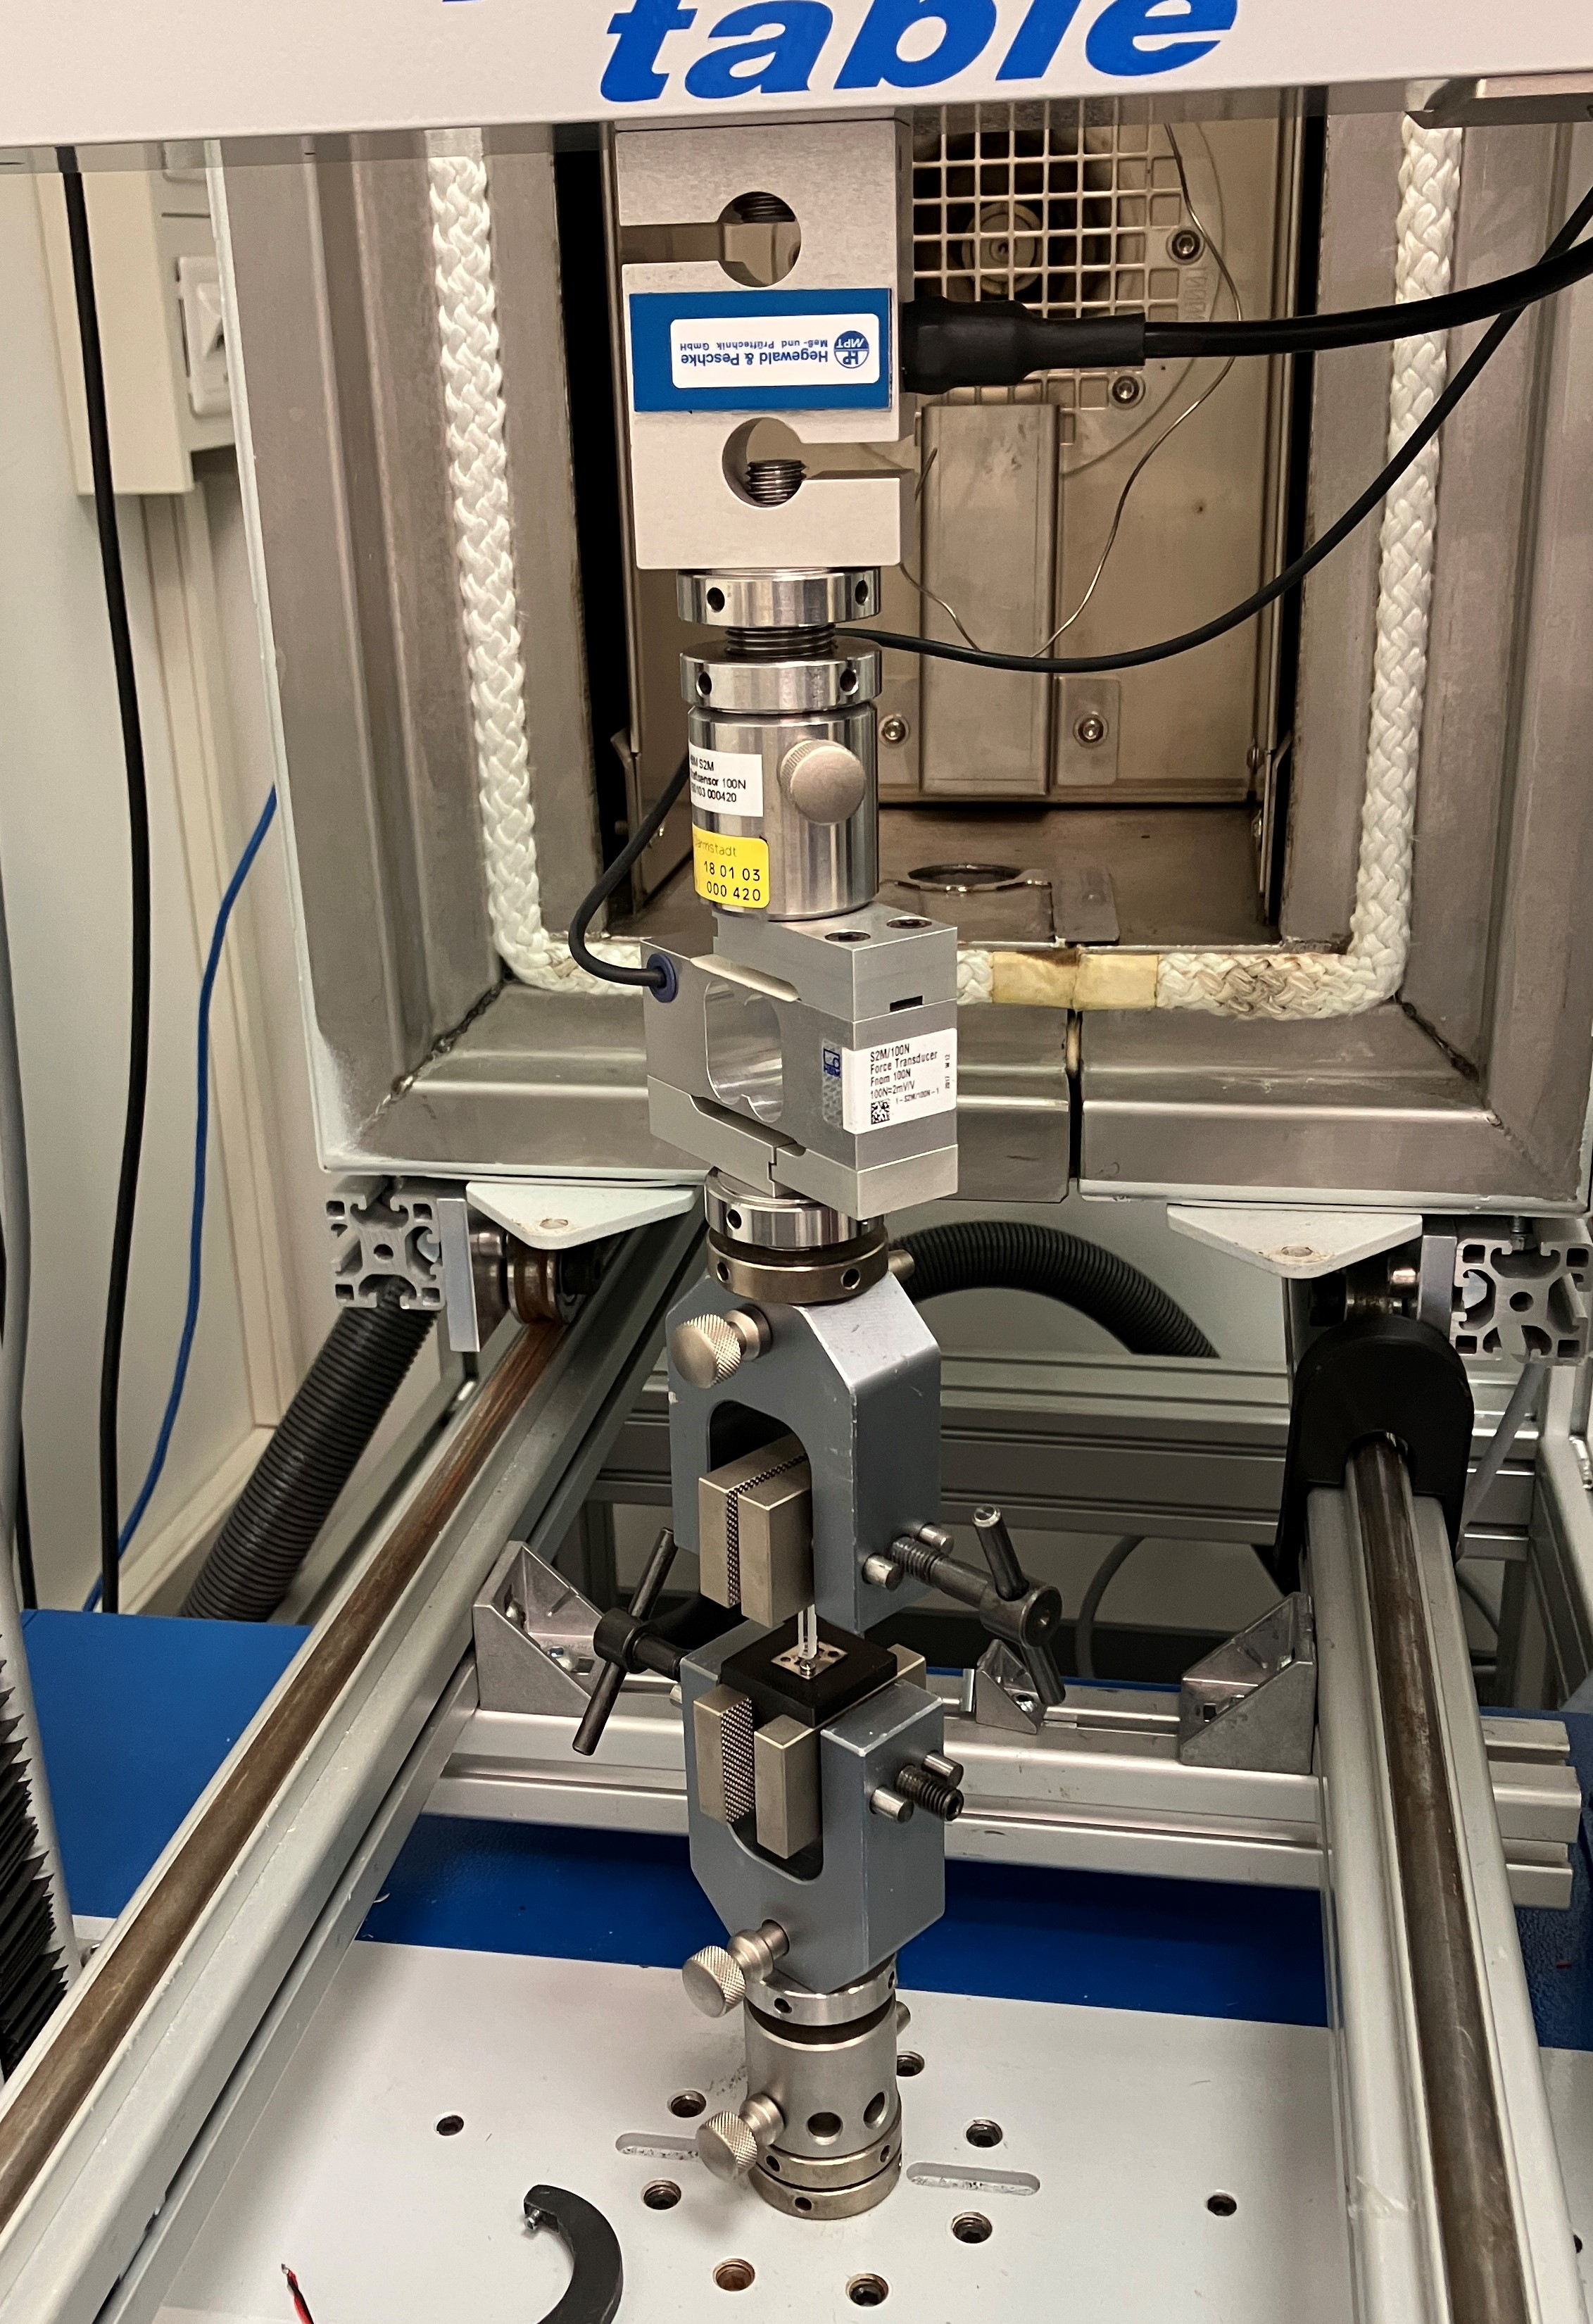
\includegraphics[width=6cm, height=9cm]{AufbauPullingMachine}
		\caption{}
	\end{subfigure}
	\begin{subfigure}[]{0.45\textwidth}
		\centering
		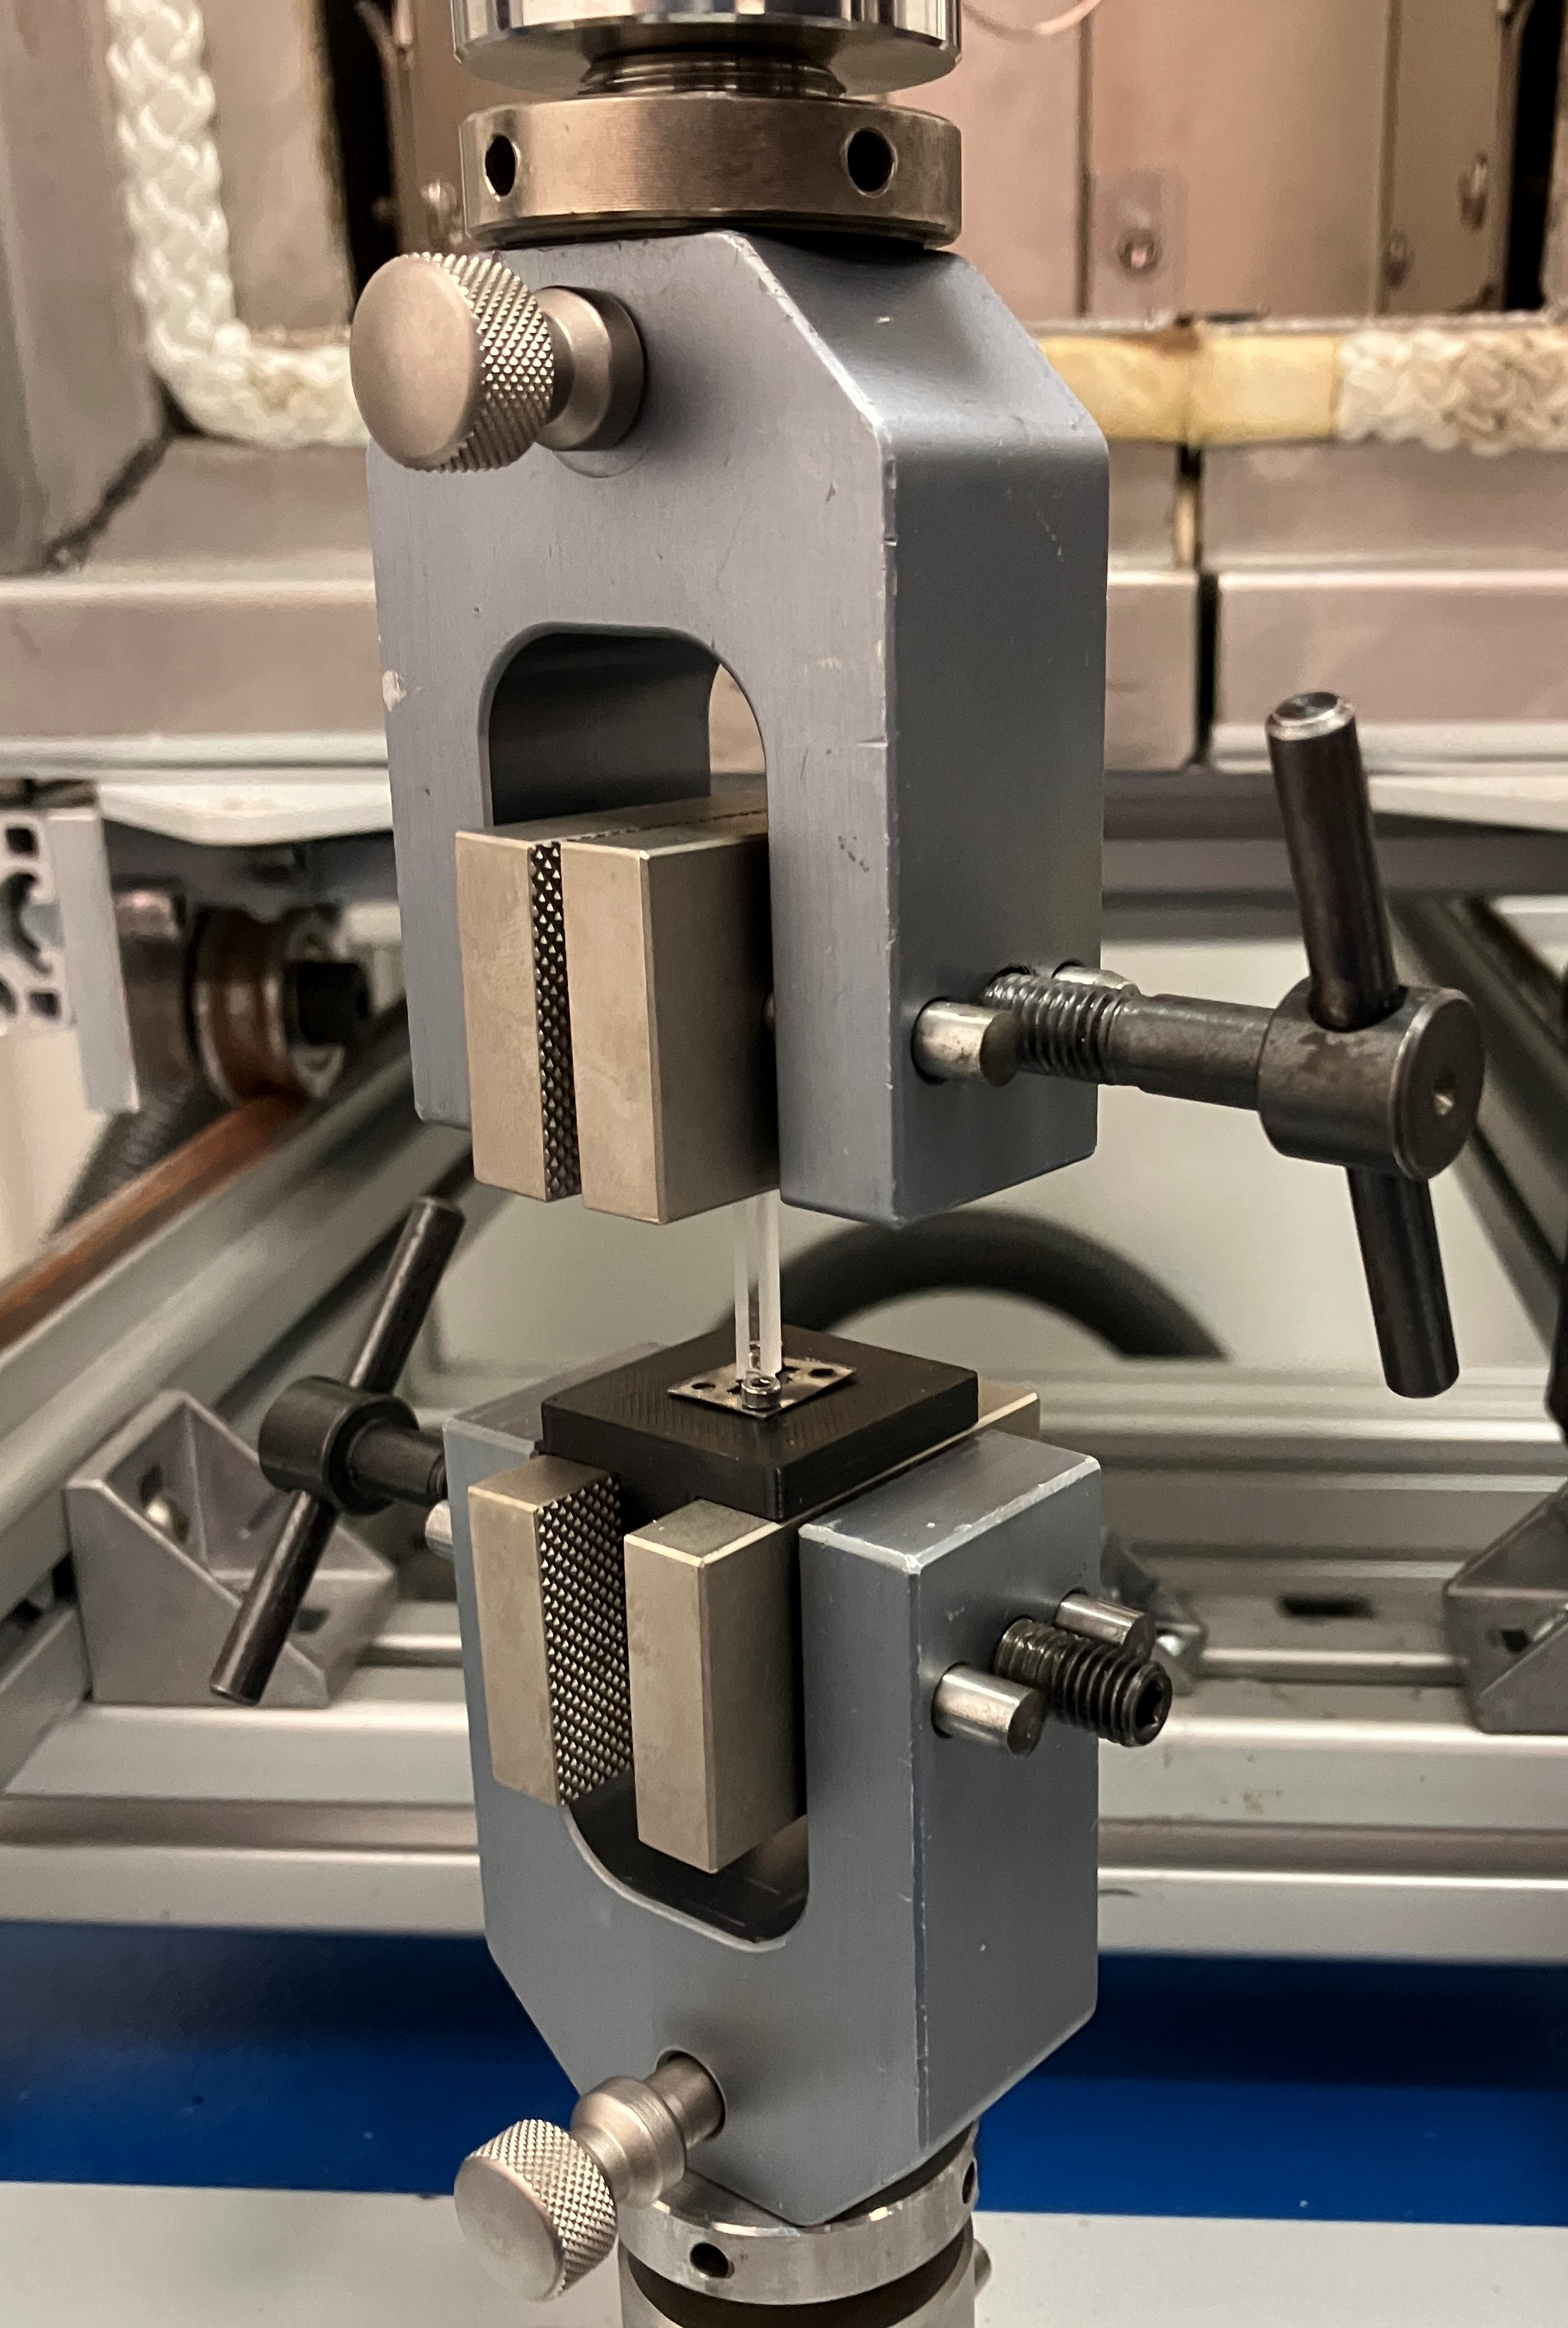
\includegraphics[width=6cm, height=9cm]{AufbauPullingMachineCloseup}
		\caption{}
	\end{subfigure}
	\caption{Setup on the Pulling Machine.}
	\label{fig:PullingMachineSetup}
\end{figure}

Because Glue dosaging varied a good amount, the Area is not assumed to be the bottom of the stamp. After Pulling, the glue is sticking on the stamp, outlining the area of the glue. The glue is analyzed under a microscope and the area is measured. With the Area and the maximum Force shortly before detaching, the Tensile stress is calculated. Then the experiment is repeated.



\subsection{detaching ice from PDMS}

1:2 and 4:1

